\documentclass{article}

\usepackage{fontspec}
\usepackage{fullpage}
\usepackage{multicol}
\usepackage{multirow}
\usepackage{tikz}

\begin{document}

\newfontfamily\swfill{SuttonSignWritingFill.ttf}
\newfontfamily\swline{SuttonSignWritingLine.ttf}
\newcommand{\bul}{\hfil$\bullet$&}
\renewenvironment{glossary}{\begin{multicols}{5}\begin{center}}{\end{center}\end{multicols}}
\setcounter{secnumdepth}{0}
\setlength{\columnseprule}{1pt}

\section{Supplement For Lesson 9}

\begin{center}
\it
Objectives inspired by, vocabulary transcribed from, and sentences and story by Bill Vicars.

Handshape photos by Adam Frost.

No endorsement implied nor given by either.
\end{center}

\subsection{Objectives}

\begin{tabular}{p{1cm}p{14cm}}
\bul I have completed the objectives for this lesson.\\
\bul I know which base symbols are in Symbol Groups hit wall and hit floor.\\
\bul I am able to read, write, and sign the ASL handshapes in symbol group five.\\
\bul I am able to recognize the vocabulary for this lesson.\\
\bul I am able to read the practice sentences for this lesson.\\
\bul I am able to read the practice story for this lesson.\\
\end{tabular}

\subsection{Symbol Groups Hit Wall and Hit Floor}

The seventeenth Symbol Group we informally call hit wall, though it's official name is ``Curves Hit Wall Plane''.

\begin{center}
\begin{tabular}{rcrc}
\textbf{Base Symbol}&\textbf{Example}&\textbf{Base Symbol}&\textbf{Example}\\
Curve Hits Front Wall               &B509x512S2a600492x489&Hump Hits Front Wall           &B509x518S2a700491x483\\
Loop Hits Front Wall                &B512x524S2a800488x477&Wave Hits Front Wall           &B509x516S2a900492x485\\
Rotation Single Hits Front Wall     &B514x512S2aa00486x489&Rotation Double Hits Front Wall&B518x512S2ab00482x489\\
Rotation Alternating Hits Front Wall&B520x513S2ac00480x488&Curve Hits Chest               &B507x512S2ad00494x489\\
Hump Hits Chest                     &B507x518S2ae00494x482&Loop Hits Chest                &B510x524S2af00490x477\\
Wave Hits Chest                     &B510x518S2b000491x482&Rotation Single Hits Chest     &B514x512S2b100486x489\\
Rotation Double Hits Chest          &B518x512S2b200482x489&Rotation Alternating Hits Chest&B520x513S2b300480x488\\
Wave Diagonal Path Small            &B511x519S2b400489x482&Wave Diagonal Path Medium      &B513x526S2b500487x475\\
Wave Diagonal Path Large            &B519x526S2b600481x475\\
\end{tabular}
\end{center}

The eighteenth Symbol Group we informally call hit floor, and it's official name is ``Curves Hit Floor Plane''.

\begin{center}
\begin{tabular}{rcrc}
\textbf{Base Symbol}&\textbf{Example}&\textbf{Base Symbol}&\textbf{Example}\\
Curve Hits Ceiling Small         &B510x512S2b700491x489&Curve Hits Ceiling Large       &B512x513S2b800489x487\\
Hump Hits Ceiling 2 Humps Small  &B513x512S2b900487x488&Hump Hits Ceiling 2 Humps Large&B516x517S2ba00485x484\\
Hump Hits Ceiling 3 Humps Small  &B517x516S2bb00484x484&Hump Hits Ceiling 3 Humps Large&B519x521S2bc00481x480\\
Loop Hits Ceiling Small Single   &B510x513S2bd00491x487&Loop Hits Ceiling Large Single &B511x516S2be00489x484\\
Loop Hits Ceiling Small Double   &B510x517S2bf00491x483&Loop Hits Ceiling Large Double &B511x520S2c000489x480\\
Wave Hits Ceiling Small          &B512x515S2c100489x485&Wave Hits Ceiling Large        &B516x520S2c200484x480\\
Rotation Single Hits Ceiling     &B513x512S2c300487x489&Rotation Double Hits Ceiling   &B520x512S2c400480x489\\
Rotation Alternating Hits Ceiling&B520x512S2c500480x488&Curve Hits Floor Small         &B510x513S2c600491x487\\
Curve Hits Floor Large           &B512x515S2c700489x486&Hump Hits Floor 2 Humps Small  &B512x513S2c800489x487\\
Hump Hits Floor 2 Humps Large    &B516x517S2c900485x484&Hump Hits Floor 3 Humps Small  &B515x516S2ca00486x485\\
Hump Hits Floor 3 Humps Large    &B520x522S2cb00481x479&Loop Hits Floor Small Single   &B510x513S2cc00491x487\\
Loop Hits Floor Large Single     &B511x516S2cd00489x484&Loop Hits Floor Small Double   &B510x517S2ce00490x483\\
Loop Hits Floor Large Double     &B511x520S2cf00489x480&Wave Hits Floor Small          &B512x513S2d000488x487\\
Wave Hits Floor Large            &B518x520S2d100482x481&Rotation Single Hits Floor     &B513x512S2d200487x489\\
Rotation Double Hits Floor       &B520x512S2d300481x489&Rotation Alternating Hits Floor&B522x512S2d400479x489\\
\end{tabular}
\end{center}

Before you can consider this lesson complete, you need to be able to list off the symbol groups as:
``one, two, three, four, five, six, seven, eight, nine, thumb;''
``contact, finger, wall, diagonal, floor, curve wall, hit wall, hit floor.''

Almost the last help when remembering the second set of base symbols --- curve outside, hit inside.

So we continued with the wall followed by floor, now we did two hits together because curve outside and hit inside.

It should not surprise you to know that curve floor is next.
The last symbol just has to be remembered, but that's for the next lesson.

\subsection{Remaining ASL Handshapes From Symbol Group Five}

The twenty one handshapes in Symbol Group Five used by ASL in order are:
Five Fingers Spread;
Five Fingers Spread Heel;
Five Fingers Spread, Four Bent;
Five Fingers Spread, Four Bent Heel;
Five Fingers Spread Bent;
Five Fingers Spread Bent Heel;
Five Fingers Spread Cup;
Five Fingers Spread Cup Open;
Five Fingers Spread Hinge;
Flat Hand;
Flat Heel;
Flat, Thumb Side;
Flat, Thumb Side Heel;
Cup;
{\it
Cup, Thumb Side;
Cup, No Thumb;
Circle;
Hinge;
Hinge, Thumb Side
Hinge, No Thumb
and Angle.
}

\subsubsection{The Cup, Thumb Side Handshape}

\begin{center}
\begin{tabular}{r*{6}{c}}
&\textbf{Fill 1}&\textbf{Fill 2}&\textbf{Fill 3}&\textbf{Fill 4}&\textbf{Fill 5}&\textbf{Fill 6}\\
\multirow{2}{*}{\textbf{Right}}&
B512x510S16f00488x490&
B512x510S16f10488x490&
B512x510S16f20488x490&
B512x510S16f30488x490&
B512x510S16f40488x490&
B512x510S16f50488x490\\
&
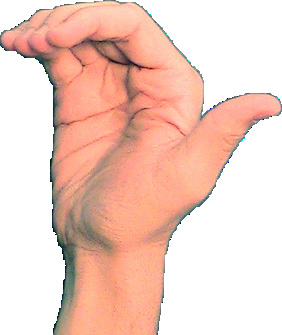
\includegraphics[scale=0.1]{images/05-15-1.jpg}&
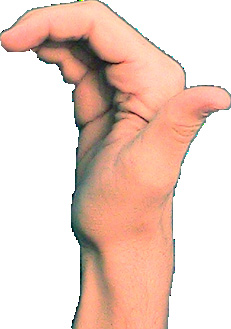
\includegraphics[scale=0.1]{images/05-15-2.jpg}&
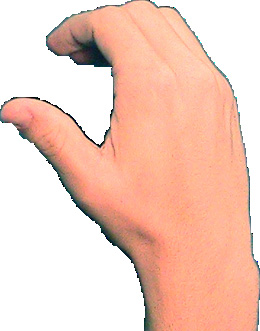
\includegraphics[scale=0.1]{images/05-15-3.jpg}&
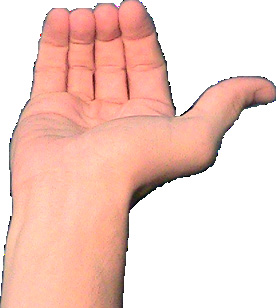
\includegraphics[scale=0.1]{images/05-15-4.jpg}&
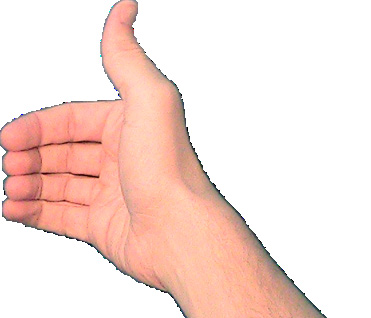
\includegraphics[scale=0.1]{images/05-15-5.jpg}&
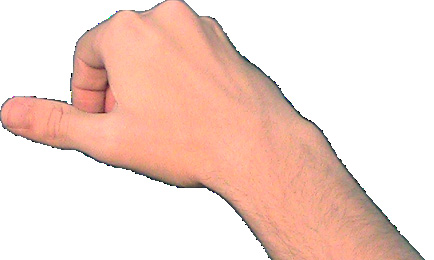
\includegraphics[scale=0.1]{images/05-15-6.jpg}\\
\textbf{Left}&
B512x510S16f08488x490&
B512x510S16f18488x490&
B512x510S16f28488x490&
B512x510S16f38488x490&
B512x510S16f48488x490&
B512x510S16f58488x490\\
\end{tabular}
\end{center}

\subsubsection{The Cup, No Thumb Handshape}

\begin{center}
\begin{tabular}{r*{6}{c}}
&\textbf{Fill 1}&\textbf{Fill 2}&\textbf{Fill 3}&\textbf{Fill 4}&\textbf{Fill 5}&\textbf{Fill 6}\\
\multirow{2}{*}{\textbf{Right}}&
B509x510S17100492x490&
B509x510S17110492x490&
B509x510S17120492x490&
B509x510S17130492x490&
B509x510S17140492x490&
B509x510S17150492x490\\
&
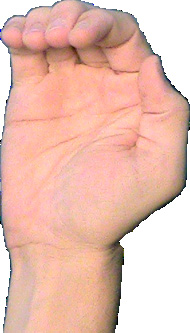
\includegraphics[scale=0.1]{images/05-16-1.jpg}&
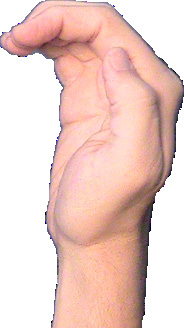
\includegraphics[scale=0.1]{images/05-16-2.jpg}&
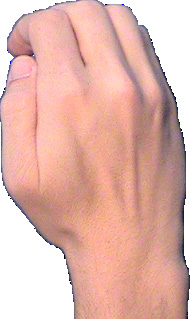
\includegraphics[scale=0.1]{images/05-16-3.jpg}&
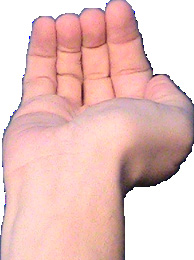
\includegraphics[scale=0.1]{images/05-16-4.jpg}&
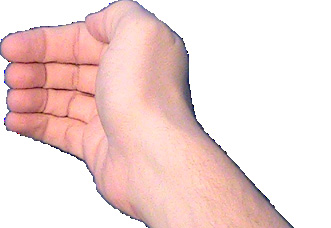
\includegraphics[scale=0.1]{images/05-16-5.jpg}&
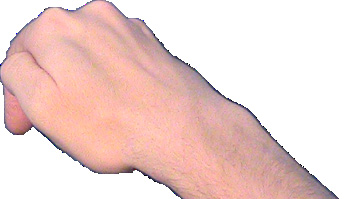
\includegraphics[scale=0.1]{images/05-16-6.jpg}\\
\textbf{Left}&
B509x510S17108492x490&
B509x510S17118492x490&
B509x510S17128492x490&
B509x510S17138492x490&
B509x510S17148492x490&
B509x510S17158492x490\\
\end{tabular}
\end{center}

\subsubsection{The Circle Handshape}

\begin{center}
\begin{tabular}{r*{6}{c}}
&\textbf{Fill 1}&\textbf{Fill 2}&\textbf{Fill 3}&\textbf{Fill 4}&\textbf{Fill 5}&\textbf{Fill 6}\\
\multirow{2}{*}{\textbf{Right}}&
B508x508S17600492x492&
B508x508S17610492x492&
B508x508S17620492x492&
B508x508S17630492x492&
B508x508S17640492x492&
B508x508S17650492x492\\
&
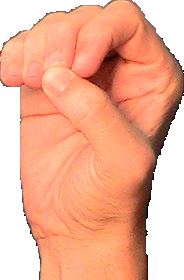
\includegraphics[scale=0.1]{images/05-17-1.jpg}&
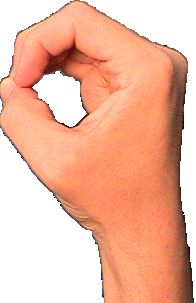
\includegraphics[scale=0.1]{images/05-17-2.jpg}&
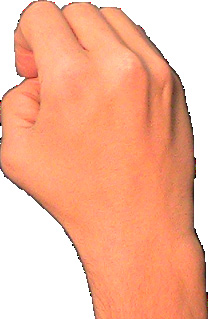
\includegraphics[scale=0.1]{images/05-17-3.jpg}&
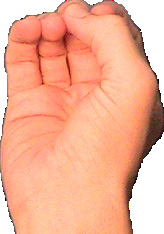
\includegraphics[scale=0.1]{images/05-17-4.jpg}&
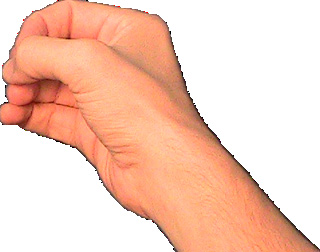
\includegraphics[scale=0.1]{images/05-17-5.jpg}&
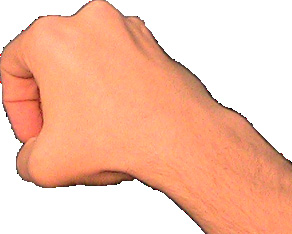
\includegraphics[scale=0.1]{images/05-17-6.jpg}\\
\textbf{Left}&
B508x508S17600492x492&
B508x508S17618492x492&
B508x508S17628492x492&
B508x508S17638492x492&
B508x508S17648492x492&
B508x508S17658492x492\\
\end{tabular}
\end{center}

\subsubsection{The Hinge Handshape}

\begin{center}
\begin{tabular}{r*{6}{c}}
&\textbf{Fill 1}&\textbf{Fill 2}&\textbf{Fill 3}&\textbf{Fill 4}&\textbf{Fill 5}&\textbf{Fill 6}\\
\multirow{2}{*}{\textbf{Right}}&
B512x508S17d00489x493&
B512x508S17d10489x493&
B512x508S17d20489x493&
B512x508S17d30489x493&
B512x508S17d40489x493&
B512x508S17d50489x493\\
&
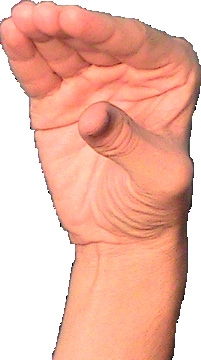
\includegraphics[scale=0.1]{images/05-18-1.jpg}&
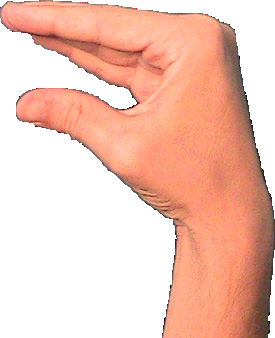
\includegraphics[scale=0.1]{images/05-18-2.jpg}&
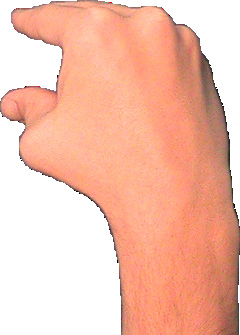
\includegraphics[scale=0.1]{images/05-18-3.jpg}&
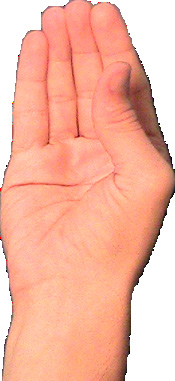
\includegraphics[scale=0.1]{images/05-18-4.jpg}&
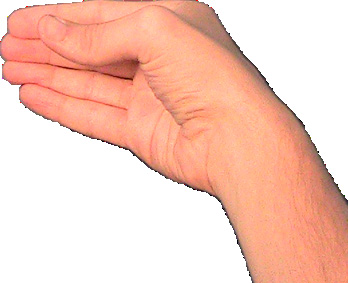
\includegraphics[scale=0.1]{images/05-18-5.jpg}&
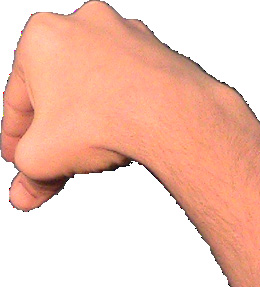
\includegraphics[scale=0.1]{images/05-18-6.jpg}\\
\textbf{Left}&
B512x508S17d08489x493&
B512x508S17d18489x493&
B512x508S17d28489x493&
B512x508S17d38489x493&
B512x508S17d48489x493&
B512x508S17d50489x493\\
\end{tabular}
\end{center}

\subsubsection{The Hinge, Thumb Side Handshape}

\begin{center}
\begin{tabular}{r*{6}{c}}
&\textbf{Fill 1}&\textbf{Fill 2}&\textbf{Fill 3}&\textbf{Fill 4}&\textbf{Fill 5}&\textbf{Fill 6}\\
\multirow{2}{*}{\textbf{Right}}&
B515x508S18000485x493&
B515x508S18010485x493&
B515x508S18020485x493&
B515x508S18030485x493&
B515x508S18040485x493&
B515x508S18050485x493\\
&
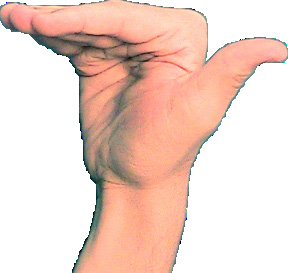
\includegraphics[scale=0.1]{images/05-19-1.jpg}&
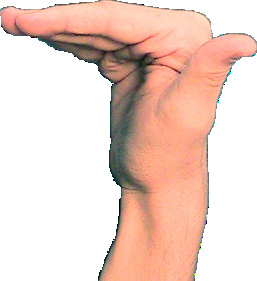
\includegraphics[scale=0.1]{images/05-19-2.jpg}&
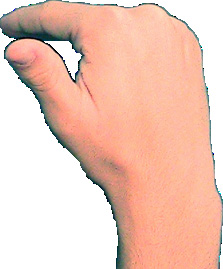
\includegraphics[scale=0.1]{images/05-19-3.jpg}&
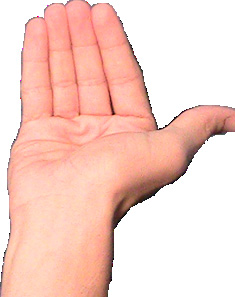
\includegraphics[scale=0.1]{images/05-19-4.jpg}&
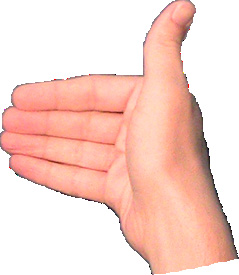
\includegraphics[scale=0.1]{images/05-19-5.jpg}&
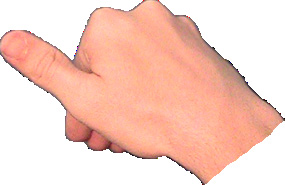
\includegraphics[scale=0.1]{images/05-19-6.jpg}\\
\textbf{Left}&
B515x508S18008485x493&
B515x508S18018485x493&
B515x508S18028485x493&
B515x508S18038485x493&
B515x508S18048485x493&
B515x508S18058485x493\\
\end{tabular}
\end{center}

\subsubsection{The Hinge, No Thumb Handshape}

\begin{center}
\begin{tabular}{r*{6}{c}}
&\textbf{Fill 1}&\textbf{Fill 2}&\textbf{Fill 3}&\textbf{Fill 4}&\textbf{Fill 5}&\textbf{Fill 6}\\
\multirow{2}{*}{\textbf{Right}}&
B512x508S18200489x493&
B512x508S18210489x493&
B512x508S18220489x493&
B512x508S18230489x493&
B512x508S18240489x493&
B512x508S18250489x493\\
&
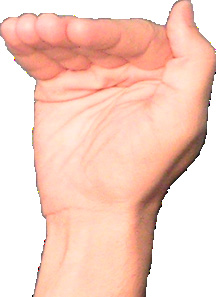
\includegraphics[scale=0.1]{images/05-20-1.jpg}&
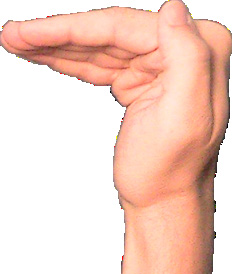
\includegraphics[scale=0.1]{images/05-20-2.jpg}&
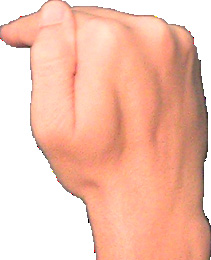
\includegraphics[scale=0.1]{images/05-20-3.jpg}&
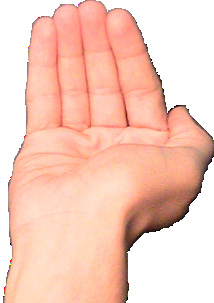
\includegraphics[scale=0.1]{images/05-20-4.jpg}&
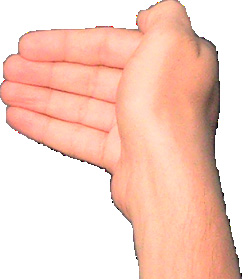
\includegraphics[scale=0.1]{images/05-20-5.jpg}&
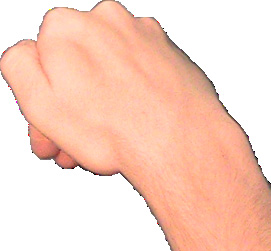
\includegraphics[scale=0.1]{images/05-20-6.jpg}\\
\textbf{Left}&
B512x508S18208489x493&
B512x508S18218489x493&
B512x508S18228489x493&
B512x508S18238489x493&
B512x508S18248489x493&
B512x508S18258489x493\\
\end{tabular}
\end{center}

\subsubsection{The Angle Handshape}

\begin{center}
\begin{tabular}{r*{6}{c}}
&\textbf{Fill 1}&\textbf{Fill 2}&\textbf{Fill 3}&\textbf{Fill 4}&\textbf{Fill 5}&\textbf{Fill 6}\\
\multirow{2}{*}{\textbf{Right}}&
B512x508S18500488x493&
B512x508S18510488x493&
B512x508S18520488x493&
B512x508S18530488x493&
B512x508S18540488x493&
B512x508S18550488x493\\
&
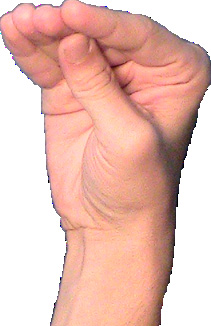
\includegraphics[scale=0.1]{images/05-21-1.jpg}&
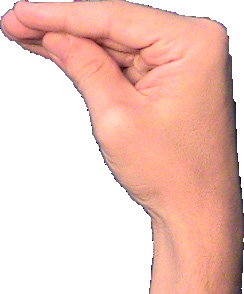
\includegraphics[scale=0.1]{images/05-21-2.jpg}&
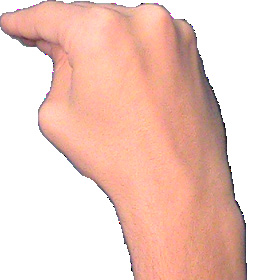
\includegraphics[scale=0.1]{images/05-21-3.jpg}&
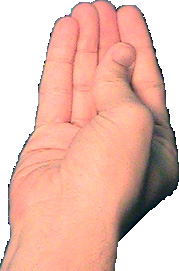
\includegraphics[scale=0.1]{images/05-21-4.jpg}&
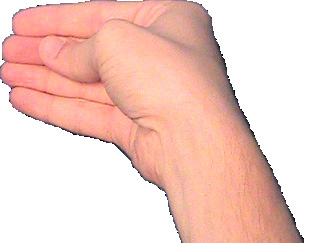
\includegraphics[scale=0.1]{images/05-21-5.jpg}&
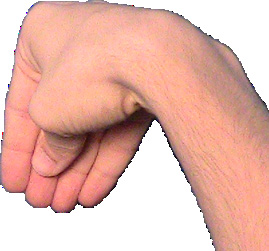
\includegraphics[scale=0.1]{images/05-21-6.jpg}\\
\textbf{Left}&
B512x508S18508488x493&
B512x508S18518488x493&
B512x508S18528488x493&
B512x508S18538488x493&
B512x508S18548488x493&
B512x508S18558488x493\\
\end{tabular}
\end{center}

\subsection{Vocabulary}

\begin{glossary}

\textbf{basement}\\
AS1f502S15a1aS2e70eM527x522S15a1a473x478S1f502479x497S2e70e502x507

\textbf{bathtub}\\
AS1f702S1f70aS22f20S21200S1fb20S11520S15a20S36d00M531x551S36d00479x449S21200487x476S1f702516x463S1f70a470x463S22f20490x497S1fb20474x532S11520493x521S15a20514x524

\textbf{close}\\
AS15a00S15a00S2df0cS2df14S2fb04S15a20S15a20M549x539S15a00452x478S15a20481x462S15a20512x462S15a00537x478S2df0c506x502S2df14475x501S2fb04495x533

\textbf{close door}\\
AS15a00S15a00S2df0cS2df14S2fb04S15a20S15a20M549x539S15a00452x478S15a20481x462S15a20512x462S15a00537x478S2df0c506x502S2df14475x501S2fb04495x533

\textbf{close window}\\
AS15a02S15a06S22a04S20500M520x524S15a02493x496S15a06488x512S20500481x497S22a04498x477

\textbf{closet}\\
AS15a20S15a28S20e00S2e004M516x535S15a20498x478S15a28484x478S2e004495x507S20e00491x465

\textbf{couch}\\
AS11820S11529S20800S20800S16d51S16d53S26606S26612S2fb04M573x552S11529475x468S11820494x472S20800485x449S20800501x449S16d51507x520S16d53474x520S26606543x523S26612427x519S2fb04490x546

\textbf{desk}\\
AS15a52S15a5aS20600S20600S37816S37816M556x513S20600534x495S20600445x496S37816473x504S37816493x492S15a52468x488S15a5a506x501

\textbf{door}\\
AS15a20S15a28S20e00S2e004M516x535S15a20498x478S15a28484x478S2e004495x507S20e00491x465

\textbf{dresser}\\
AS20330S20338S26c28M534x516S20330519x484S20338467x484S26c28488x501

\textbf{dry}\\
AS10012S26506S20e00S10612S2ff00M594x526S10012501x511S10612568x511S26506548x511S20e00533x513S2ff00482x483

\textbf{dryer}\\
AS10012S26a06S26506S20e00S10612S2ff00M594x532S10012501x511S10612568x511S26a06548x505S20e00533x513S2ff00482x483

\textbf{garage}\\
AS11e40S15a56S26a00M527x524S11e40480x494S15a56474x477S26a00500x490

\textbf{garbage}\\
AS10010S2d600S20500S37605M529x532S37605472x469S20500488x504S10010513x502S2d600494x485

\textbf{kitchen}\\
AS14050S15a37S20500S14030S15a37S20500M521x546S15a37496x523S15a37498x474S14050483x455S20500484x480S20500482x530S14030480x502

\textbf{lights}\\
AS15311S15319S18511S18519S2ff00M545x518S2ff00482x483S18511516x469S18519455x470S15311522x443S15319454x446

\textbf{microwave}\\
AS18510S18518S26c02S21b00S21600S26c1aS21b00S21600S15410S15418M594x526S18510569x499S18518406x495S26c02549x489S26c1a439x486S15410528x488S15418462x486S21b00552x477S21600553x518S21b00444x475S21600445x515

\textbf{open}\\
AS15a20S15a20S20500S2df04S2df1cM523x533S15a20488x481S15a20502x481S2df04502x512S2df1c478x512S20500496x468

\textbf{open door}\\
AS14720S14728S2e004M519x527S14720499x473S14728482x473S2e004498x499

\textbf{open window}\\
AS15a02S15a0aS22a00M514x522S15a02487x496S15a06487x510S22a00495x478

\textbf{refrigerator}\\
AS11a20S14a20S1ce20M530x515S11a20470x485S14a20490x500S1ce20508x485

\textbf{shower}\\
AS20311S22f03S21d01S2ff00M545x518S2ff00482x483S20311524x455S22f03512x467S21d01517x448

\textbf{sink}\\
AS20320S19220S11920S14020M555x516S19220473x496S20320445x500S11920497x490S14020526x485

\textbf{stove}\\
AS20320S1fb20S17620S10e20S14a20M554x516S20320447x498S1fb20468x494S17620490x499S10e20516x484S14a20539x501

\textbf{table}\\
AS15a52S15a5aS20600S20600S37816S37816M556x513S20600534x495S20600445x496S37816473x504S37816493x492S15a52468x488S15a5a506x501

\textbf{window}\\
AS15a02S15a06S20500S23600M522x529S15a02495x504S15a06489x517S20500494x491S23600479x472

\textbf{yesterday}\\
AS1f527S20500S22a00S20500S2ff00M537x541S20500519x485S1f527503x519S20500517x511S2ff00482x483S22a00524x496

\end{glossary}

\subsection{Practice Sheet 9.A}

\begin{multicols}{5}
\begin{center}

M508x515S10000493x485 % 1
M536x504S38800464x496 % .
M518x518S30a00482x483 % y/n
M510x523S10040495x493S26500491x478 % you
M520x522S1f502505x498S1f50a480x498S22a20493x478 % live
M527x522S15a1a473x478S1f502479x497S2e70e502x507 % basement
M510x508S1f720490x493 % a
M516x512S14021485x488 % p
M508x510S1fb20493x491 % t
M536x507S38900464x493 % ?
\vfil
\columnbreak

M508x515S10e00493x485 % 2
M536x504S38800464x496 % .
R531x531S36d00479x469S21200487x496S1f702516x483S1f70a470x483S22f20490x517 % bath
L545x518S2ff00482x483S20311524x455S22f03512x467S21d01517x448 % shower
M537x504S38700463x496 % ,
M518x518S30c00482x483 % \?
M540x543S1c507499x518S20600518x508S2ff00482x483 % favorite
M535x526S2fb04491x520S1f502512x474S23100509x503S23110465x505S1f502471x474 % which
M536x507S38900464x493 % ?
\vfil
\columnbreak

M512x515S11e00489x485 % 3
M536x504S38800464x496 % .
M518x518S30a00482x483 % y/n
M507x523S15a28494x496S26500493x477 % your
M518x520S1fb20482x490S27106503x480 % bathroom
M532x518S18049468x483S18041507x483S20500486x507S20500504x507 % have
M508x510S1fb20493x491 % t
M508x515S11520493x485 % u
M507x511S14720493x489 % b
M536x507S38900464x493 % ?
\vfil
\columnbreak

M511x516S14400489x485 % 4
M536x504S38800464x496 % .
M518x518S30a00482x483 % y/n
M510x523S10040495x493S26500491x478 % you
M522x525S1f748479x496S1f740502x496S20500496x514S26a20490x475 % together
M516x525S10000492x495S2e806484x475 % someone
M536x507S38900464x493 % ?
\vfil
\columnbreak

M512x516S14c00489x485 % 5
M536x504S38800464x496 % .
M507x523S15a28494x496S26500493x477 % your
M573x552S11529475x468S11820494x472S20800485x449S20800501x449S16d51507x520S16d53474x520S26606543x523S26612427x519S2fb04490x546 % couch
M537x504S38700463x496 % ,
M518x518S30c00482x483 % \?
M518x565S14c00488x534S22520484x520S2ff00482x483 % color
M536x507S38900464x493 % ?
\vfil

\end{center}
\end{multicols}

\subsection{Practice Sheet 9.B}

\begin{multicols}{5}
\begin{center}

M509x515S18720491x486 % 6
M536x504S38800464x496 % .
M518x518S30a00482x483 % y/n
M527x524S11e40480x494S15a56474x477S26a00500x490 % garage
M532x518S18049468x483S18041507x483S20500486x507S20500504x507 % have
M536x507S38900464x493 % ?
\vfil
\columnbreak

M511x514S1a520490x486 % 7
M536x504S38800464x496 % .
M518x518S30a00482x483 % y/n
M556x537S20301466x474S20301511x464S28800527x500S2880c510x500S2880c544x500S28814464x501S28818445x501S28818482x502S2fb04496x531 % car
M532x518S18049468x483S18041507x483S20500486x507S20500504x507 % have
M536x507S38900464x493 % ?
M518x518S30c00482x483 % \?
M526x535S22a20494x501S14c08474x465S14c00503x465S20338478x520S20330508x520 % how many
M516x535S15a20498x478S15a28484x478S2e004495x507S20e00491x465 % door
M536x507S38900464x493 % ?
\vfil
\columnbreak

M511x514S1bb20490x486 % 8
M536x504S38800464x496 % .
M507x523S15a28494x496S26500493x477 % your
M525x539S15a11502x476S15a19476x476S20500495x462S23904505x501S2391c477x501S2fb04494x533 % house
M537x504S38700463x496 % ,
M529x532S37605472x469S20500488x504S10010513x502S2d600494x485 % garbage
M518x518S30c00482x483 % \?
M518x540S34600482x483S1e111473x512S21800463x502 % who
M549x550S20311528x514S20315497x529S22b21493x491S14c11487x450S14c1f451x475 % throw out (mime)
M536x507S38900464x493 % ?
\vfil
\columnbreak

M511x515S1ce20489x485 % 9
M536x504S38800464x496 % .
M507x523S15a28494x496S26500493x477 % your
M594x532S10012501x511S10612568x511S26a06548x505S20e00533x513S2ff00482x483 % dryer
M537x504S38700463x496 % ,
R515x508S1f000486x493 % g
R510x508S1f720490x493 % a
R508x508S20320493x493 % s
L533x525S10642507x510S1064a468x509S26a02507x476S26a16482x475S20602495x487 % battery
M518x518S30c00482x483 % \?
M535x526S2fb04491x520S1f502512x474S23100509x503S23110465x505S1f502471x474 % which
M536x507S38900464x493 % ?
\vfil
\columnbreak

M513x528S2a538494x472S1f540488x504 % 10
M536x504S38800464x496 % .
M515x519S10047485x498S26507501x481 % 3rd person
M556x513S20600534x495S20600445x496S37816473x504S37816493x492S15a52468x488S15a5a506x501 % table
M537x504S38700463x496 % ,
M518x518S30c00482x483 % \?
M518x565S14c00488x534S22520484x520S2ff00482x483 % color
M536x507S38900464x493 % ?
\vfil

\end{center}
\end{multicols}

\subsection{Practice Sheet 9.C}

\begin{multicols}{5}
\begin{center}

M512x520S10000489x490S21d00494x480 % 11
M536x504S38800464x496 % .
M528x566S34700482x483S10012498x520S27102495x526 % brush teeth
M525x526S1001a475x511S1ea51489x474S26606495x496S21100477x494 % paste ???
M510x523S10040495x493S26500491x478 % you
M537x504S38700463x496 % ,
M518x518S30c00482x483 % \?
M524x532S14249491x508S14240477x480S2e800510x469S20500480x509 % kind
M536x507S38900464x493 % ?
\vfil
\columnbreak

M509x521S10e00491x491S21d00491x480 % 12
M536x504S38800464x496 % .
M510x523S10040495x493S26500491x478 % you
M540x543S1c507499x518S20600518x508S2ff00482x483 % favorite
R508x508S20320493x493 % s
R508x510S1fb20493x491 % t
R508x508S17620492x492 % o
R508x515S10e20493x485 % v
R508x508S14a20493x493 % e
L594x526S18510569x499S18518406x495S26c02549x489S26c1a439x486S15410528x488S15418462x486S21b00552x477S21600553x518S21b00444x475S21600445x515 % microwave
M535x526S2fb04491x520S1f502512x474S23100509x503S23110465x505S1f502471x474 % which
M536x507S38900464x493 % ?
\vfil
\columnbreak

M513x519S22114487x481S12d00489x489 % 13
M536x504S38800464x496 % .
M507x523S15a28494x496S26500493x477 % your
M508x515S11a20493x485 % r
M508x508S14a20493x493 % e
M511x515S1ce20489x485 % f
M537x504S38700463x496 % ,
M518x518S30c00482x483 % \?
M518x565S14c00488x534S22520484x520S2ff00482x483 % color
M536x507S38900464x493 % ?
\vfil
\columnbreak

M513x515S14700493x493S22114487x486 % 14
M536x504S38800464x496 % .
M549x518S15426523x479S2ff00482x483S2e000528x444S1542e451x478S2e018456x445S2fb00494x455 % ambulance
M537x504S38700463x496 % ,
M518x518S30a00482x483 % y/n
M547x530S36d00479x487S15d00528x470S26604527x500 % past
M510x523S10040495x493S26500491x478 % you
M536x507S38900464x493 % ?
\vfil
\columnbreak

M513x518S22114487x483S15d00494x491 % 15
M536x504S38800464x496 % .
M544x531S20500509x515S10011523x501S20500520x488S2ff00482x483 % deaf
M540x543S1c507499x518S20600518x508S2ff00482x483 % favorite
M521x546S15a37496x523S15a37498x474S14050483x455S20500484x480S20500482x530S14030480x502 % kitchen
M537x504S38700463x496 % ,
M574x535S22a05540x506S15d11520x488S19a37551x508S30c00482x483 % why?
M536x507S38900464x493 % ?
\vfil

\end{center}
\end{multicols}

\subsection{Practice Sheet 9.D}

\begin{multicols}{5}
\begin{center}

M520x522S18700502x492S2e00e480x479 % 16
M536x504S38800464x496 % .
M518x518S30a00482x483 % y/n
M537x541S20500519x485S1f527503x519S20500517x511S2ff00482x483S22a00524x496 % yesterday
M510x523S10040495x493S26500491x478 % you
M545x518S2ff00482x483S20311524x455S22f03512x467S21d01517x448 % shower
M536x507S38900464x493 % ?
\vfil
\columnbreak

M522x522S1a500501x494S2e00e478x478 % 17
M536x504S38800464x496 % .
M507x523S15a28494x496S26500493x477 % your
M508x508S20320493x493 % s
M511x510S19220490x491 % i (letter)
M511x513S11920490x487 % n
M515x515S14020486x485 % k
M537x504S38700463x496 % ,
M518x518S30c00482x483 % \?
M518x565S14c00488x534S22520484x520S2ff00482x483 % color
M536x507S38900464x493 % ?
\vfil
\columnbreak

M523x522S1bb00502x492S2e00e478x479 % 18
M536x504S38800464x496 % .
M507x523S15a28494x496S26500493x477 % your
M548x531S1800b517x506S18003465x506S22f00523x474S22f10450x474S20e00530x491S20e00457x491S36d10479x470 % pants
M537x504S38700463x496 % ,
M510x523S10040495x493S26500491x478 % you
M522x531S2b720489x469S18527503x504S1852f479x503 % put
R534x516S20330519x484S20338467x484S26c28488x501 % dresser
L526x534S10620495x508S2b700507x486S1004a474x484S20800505x467 % hang up ???
M518x518S30c00482x483 % \?
M535x526S2fb04491x520S1f502512x474S23100509x503S23110465x505S1f502471x474 % which
M536x507S38900464x493 % ?
\vfil
\columnbreak

M524x522S1ce00502x490S2e00e477x479 % 19
M536x504S38800464x496 % .
M518x518S30a00482x483 % y/n
M507x523S15a28494x496S26500493x477 % your
M539x593S15a17509x507S2ff00482x483S20500520x492S15a40512x541S15a48482x539S22104527x544S22104466x544S18048464x576S18040507x578 % bedroom
M532x518S18049468x483S18041507x483S20500486x507S20500504x507 % have
M522x529S15a02495x504S15a06489x517S20500494x491S23600479x472 % window
M536x507S38900464x493 % ?
\vfil
\columnbreak

M517x513S22114484x488S1f420488x498 % 20
M536x504S38800464x496 % .
M507x523S15a28494x496S26500493x477 % your
M537x504S38700463x496 % ,
M518x518S30c00482x483 % \?
M526x535S22a20494x501S14c08474x465S14c00503x465S20338478x520S20330508x520 % how many
M518x520S1fb20482x490S27106503x480 % bathroom
M536x507S38900464x493 % ?
\vfil

\end{center}
\end{multicols}

\subsection{Story 9}

\begin{multicols}{5}
\begin{center}
M537x541S20500519x485S1f527503x519S20500517x511S2ff00482x483S22a00524x496 % yesterday
M520x546S15a37481x523S1f502485x486S20500488x509S28929493x455 % help (I to 3rd)
M538x568S1dc51508x466S1dc4a490x544S1dc42464x526S20500475x553S22b03501x512S2ff00482x483 % brother
M533x522S18557514x479S1855f467x480S2892a486x507 % move
M536x504S38800464x496 % .

M515x519S10047485x498S26507501x481 % 3rd person
M547x530S36d00479x487S15d00528x470S26604527x500 % past
M520x522S1f502505x498S1f50a480x498S22a20493x478 % live
M527x522S15a1a473x478S1f502479x497S2e70e502x507 % basement
M510x508S1f720490x493 % a
M516x512S14021485x488 % p
M508x510S1fb20493x491 % t
M536x504S38800464x496 % .

M535x522S22f14466x501S22f04510x501S2fb04494x516S18215468x479S1821d508x479 % now
M525x539S15a11502x476S15a19476x476S20500495x462S23904505x501S2391c477x501S2fb04494x533 % house
M521x517S1f710479x502S26a07500x483 % itself
M536x504S38800464x496 % .

M525x539S15a11502x476S15a19476x476S20500495x462S23904505x501S2391c477x501S2fb04494x533 % house
M526x528S15a18476x472S15a10514x472S2fb00492x504S26502511x513S26516474x514 % small
M536x504S38800464x496 % .

M527x524S11e40480x494S15a56474x477S26a00500x490 % garage
M508x508S17610492x492 % zero
M536x504S38800464x496 % .

M508x508S20320493x493 % s
M508x510S1fb20493x491 % t
M508x508S17620492x492 % o
M508x515S10e20493x485 % v
M508x508S14a20493x493 % e
M537x504S38700463x496 % ,
M508x515S11a20493x485 % r
M508x508S14a20493x493 % e
M511x515S1ce20489x485 % f
M537x504S38700463x496 % ,
M561x526S15411493x474S1541f484x493S2c500521x479S2c514440x501 % washing machine
M537x504S38700463x496 % ,
M594x532S10012501x511S10612568x511S26a06548x505S20e00533x513S2ff00482x483 % dryer
M537x504S38700463x496 % ,
M556x513S20600534x495S20600445x496S37816473x504S37816493x492S15a52468x488S15a5a506x501 % table
M537x504S38700463x496 % ,
M594x526S18510569x499S18518406x495S26c02549x489S26c1a439x486S15410528x488S15418462x486S21b00552x477S21600553x518S21b00444x475S21600445x515 % microwave
M520x551S2e700504x483S15d09481x520S20500505x513S15d01493x528S15a20508x450 % all
M529x524S16d48472x504S20710495x501S18512482x476 % in
M521x546S15a37496x523S15a37498x474S14050483x455S20500484x480S20500482x530S14030480x502 % kitchen
M536x504S38800464x496 % .

M508x508S20320493x493 % s
M511x510S19220490x491 % i (letter)
M511x513S11920490x487 % n
M515x515S14020486x485 % k
M522x552S15a02495x527S15a06489x540S20500494x514S23600479x495S23a07493x449 % window above and over
M519x517S1f70f482x496S21100506x487S1f721482x484 % wash with hands
M530x515S1ed40504x486S1ed48471x486S2f900517x510S2f900474x510 % dishes
M525x517S20350510x483S20350476x483S22a24494x502 % can
M518x564S26500492x549S1e301486x518S2ff00482x483 % observe
M522x525S15a50478x475S22a04483x510S2d508500x511 % children
M534x528S19a10506x508S19a18467x508S2fb00492x473S2e010469x478S2e008509x477 % play
M519x517S1f70f482x496S21100506x487S1f721482x484 % wash with hands
M530x515S1ed40504x486S1ed48471x486S2f900517x510S2f900474x510 % dishes
M536x504S38800464x496 % .

M518x520S1fb20482x490S27106503x480 % bathroom
M526x528S15a18476x472S15a10514x472S2fb00492x504S26502511x513S26516474x514 % small
M537x504S38700463x496 % ,
M531x531S36d00479x469S21200487x496S1f702516x483S1f70a470x483S22f20490x517 % bath
M508x510S1fb20493x491 % t
M508x515S11520493x485 % u
M507x511S14720493x489 % b
M516x525S10000492x495S2e806484x475 % single
M537x504S38700463x496 % ,
M531x562S18049467x527S18041506x527S20500485x551S20500503x551S30322482x476 % don't have
M545x518S2ff00482x483S20311524x455S22f03512x467S21d01517x448 % shower
M536x504S38800464x496 % .

M539x593S15a17509x507S2ff00482x483S20500520x492S15a40512x541S15a48482x539S22104527x544S22104466x544S18048464x576S18040507x578 % bedroom
M532x518S18049468x483S18041507x483S20500486x507S20500504x507 % have
M534x516S20330519x484S20338467x484S26c28488x501 % dresser
M536x504S38800464x496 % .

M520x522S1f502505x498S1f50a480x498S22a20493x478 % live
M538x527S15a40511x475S15a48481x473S22104526x478S22104465x478S18048463x510S18040506x512 % room
M532x518S18049468x483S18041507x483S20500486x507S20500504x507 % have
M573x552S11529475x468S11820494x472S20800485x449S20800501x449S16d51507x520S16d53474x520S26606543x523S26612427x519S2fb04490x546 % couch
M537x504S38700463x496 % ,
M508x510S1fb20493x491 % t
M508x515S10e20493x485 % v
M537x504S38700463x496 % ,
M522x529S15a02495x504S15a06489x517S20500494x491S23600479x472 % window
M526x528S15a18476x472S15a10514x472S2fb00492x504S26502511x513S26516474x514 % small
M537x504S38700463x496 % ,
M534x542S10021504x473S10029467x475S24302501x502S2432a471x503S2fb00494x490S20500496x459S20500495x531 % descriptive square of smallness
M536x504S38800464x496 % .

\end{center}
\end{multicols}

\end{document}

